% latex thesis.tex  
% dvips -o thesis.ps thesis.dvi 
% ps2pdf thesis.ps 
% bibtex thesis

\def\baselinestretch{1}
\chapter{Introduction}
\def\baselinestretch{1.66}



%%%~~~~~~~~~~~~~~~~~~~~~~~~~~~~~~~~~~

Research may start from definite problems whose importance it
recognizes and whose solution is sought more or less directly with all
forces. But equally legitimate is the other method of research which
only selects the field of his activity and, contrary to the first
method, freely reconnoiters in the search for problems which are
capable of solution. 


\cite{mckay:1981:pgi}

\cite{rosenetal:1999:hodacm}

\cite{bangjensenandgutin:2000:dtaaa}

Different individuals will hold different views as
to the relative values of these two methods. If the first method leads
to greater penetration it is also easily exposed to the danger of
unproductivity. To the second method we owe the acquisition of large
and new fields in which the details of many things remain to be
determined and explored by the first method.

$2-3$

$\frac{1}{2}$ 


\begin{equation}
\frac{2}{3}
\end{equation}


\begin{equation*}
\frac{2}{3}
\end{equation*}






\begin{table}[t!]
\begin{center}
\begin{small}
\begin{tabular}{|c|c|c|c|c|c|c|}
\hline 
\multicolumn{7}{|c|}{Hyperline sequences of $S$} \\  
\hline
\hline
 4 & 2 & 4 & 3 & 5 & 6 & 7 \\ \hline
 2 & 1 & $\overline{3}$ & $\overline{6}$ & $\overline{5}$ & $\overline{7}$ & $\overline{4}$ \\ \hline
 3 & 1 & 4 & 2 & $\overline{6}$ & $\overline{7}$ & $\overline{5}$ \\ \hline
 4 & 1 & $\overline{3}$ & $\overline{6}$ & $\overline{5}$ & $\overline{7}$ & 2 \\ \hline
 5 & 1 & $\overline{6}$ & 4 & 2 & $\overline{7}$ & 3 \\ \hline
 6 & 1 & 5 & 4 & 2 & 3 & $\overline{7}$ \\ \hline
 7 & 1 & 4 & 2 & 5 & 3 & 6 \\ \hline
\end{tabular}
\end{small}
\end{center}
\caption{Hyperline sequences of the planar point configurations $S$}
\end{table}





\begin{figure}[t!]
\begin{center}
\psfrag{A}[l]{$A$}
\psfrag{B}[l]{$B$}
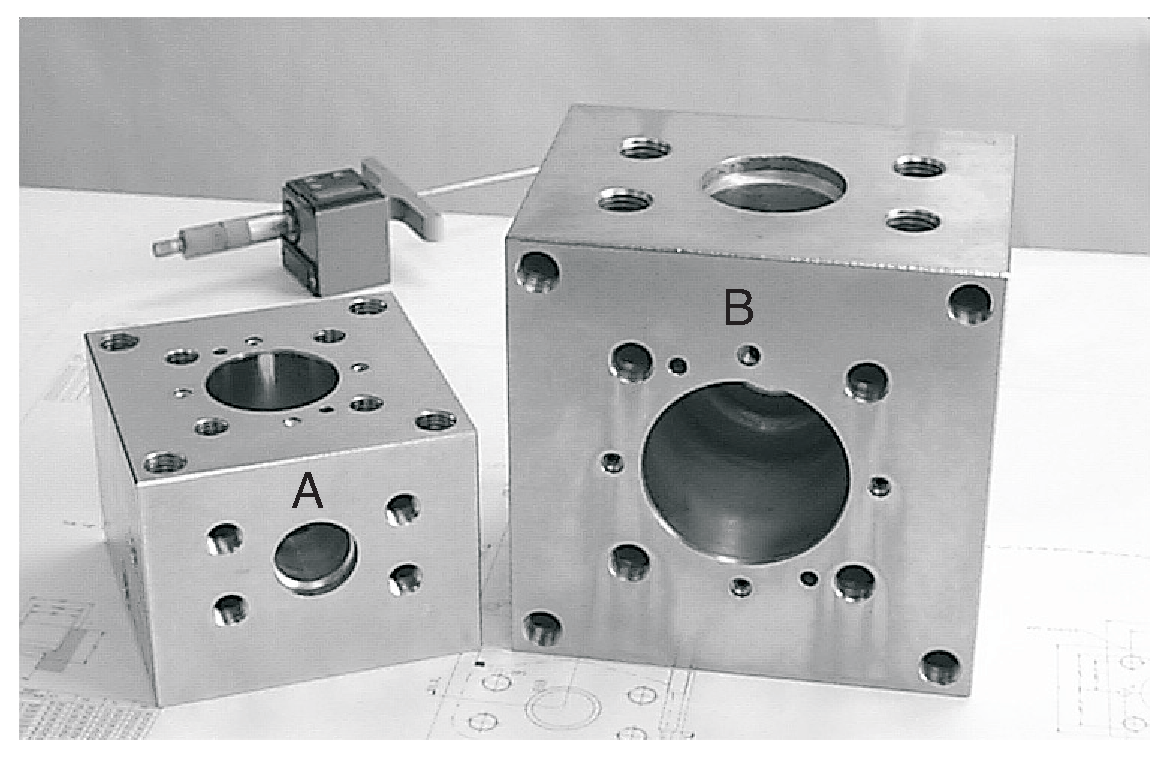
\includegraphics[width=0.99\columnwidth]{../eps/cubos.eps} 
\caption{
Images of the objects used for the experiments 
}
\label{fig:objects}
\end{center}
\end{figure}




